% chapters/intro.tex
\chapter{Introduction}
\label{ch:introduction}

% ---------- Chapter 1: Introduction ----------

\begin{figure}
\centering

\begin{subfigure}{0.45\textwidth}
  \centering
  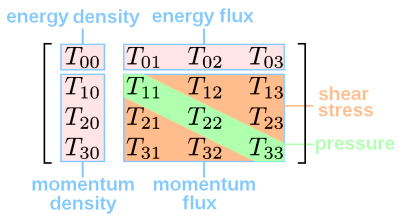
\includegraphics[width=.8\textwidth]{figures/chapter1/fig1.1}
  \caption{The general stress-energy tensor.}
  \label{fig:stress-energy-general}
\end{subfigure}
\hfill
\begin{subfigure}{0.45\textwidth}
  \centering
  \[
  \begin{pmatrix}
    c^{2} \rho{} & 0 & 0 & 0 \\
    0 & p & 0 & 0 \\  
    0 & 0 & p & 0\\
    0 & 0 & 0 & p
  \end{pmatrix}
  \]
  \caption{Perfect fluid case.}
  \label{fig:stress-energy-perfect}
\end{subfigure}
\caption{The stress-energy-momentum tensor for the general case and a perfect fluid.}
\label{fig:1.1}
\end{figure}

\begin{figure}
\centering
    \staticfigure[0.75\textwidth]{figures/chapter1/fig1.2.png}{SNe classes based on spectroscopy, with well-known examples of each class. Type Ia are thought to be the result of thermonuclear explosions, whereas all other types are caused by core collapse in massive stars. Type IIb are a crossover class, initially appearing as Type II but evolving into Type Ib/c. Image credit: Fig. 1 in \cite{Leibundgut2008}.}
\end{figure}

\begin{figure}
\centering
    \staticfigure[0.75\textwidth]{figures/chapter1/figure1.3.jpeg}{Type Ia SNe formation. This shows a singly-degenerate supernova, in which the white dwarf accretes matter from a companion star. The dwarf eventually reaches the Chandrasekhar limit, at which point its mass is too great for the dwarf to remain stable and it implodes.  Image credit: Fig. 10 of \cite{Matteucci2008}.}
\end{figure}

% CHAPTER TEXT  ----------------------------------------

Dark energy is one of the most important and least understood components of the universe. Its first introduction was the inclusion of the cosmological constant in Einstein’s equation of general relativity. Ironically, astronomical observations which indicated an expanding universe caused firstly the removal of the constant \cite{Harrison1993} and then its reintroduction \cite{Hobson2006}. Re-interpretation of the cosmological constant as a form of energy (rather than an independent scalar parameter) lead to the proposal of a broader class of ”anti-gravity fluids” which are now known as dark energy \cite{Hobson2006}. Attempts to differentiate between competing dark energy models have lead cosmologists to widen their search for evidence of expansion: the first hint of dark energy came from studies of Type Ia supernovae \cite{Leibundgut2008} but now studies (e.g. \cite{Amanullah2010,LewisBridle2002}) combine data from a variety of sources including supernovae \cite{Hicken2009,Riess2007,Kowalski2008}, the cosmic microwave background (\cmb{}), \cite{LewisBridle2002} and baryon acoustic oscillations (BAO) \cite{Komatsu2010}. 

This thesis aims to use Bayesian analysis to investigate the usefulness of Type Ia supernovae as dark energy probes. Markov Chain Monte Carlo methods are applied to determine constraints from Ia SNe on four cosmological parameters: the fractional density of matter, the (two-parameter) dark energy equation of state and the interaction constant. (The Hubble constant is included as an additional free parameter.) The data sets used in the \mcmc{} method come from three sources: observational data calibrated and processed by supernova survey groups, the same data sets with reduced errors (to investigate how uncertainties in the cosmological parameters scale with uncertainties in the observational data) and two projected sets based upon a recently-proposed, space-based survey. There is ample scope for further work in observational, computational and theoretical areas, a brief discussion of which concludes the thesis.

\section{Cosmological background}
\label{sec:cosmological-background}

The framework of modern cosmology depends upon the cosmological principle. The is an indemonstrable assumption that at a given time the universe is, apart from local irregularities, the same at all points in space. We can only prove directly that the universe is isotropic about our location. Therefore, rather than proving that the universe is isotropic and homogeneous everywhere, we must show that homogeneity is likely by demonstrating the gross improbability of a ”preferred location” which alone is isotropic \cite{Harrison1993}. Once homogeneity is established, the cosmological principle follows directly: the universe is everywhere (and everywhen) homogeneous and isotropic. Only once we have made this assumption can we propose that the laws of physics are the same at all times and places. We can now use the entire observable universe as a laboratory: if a theory can be proven false by a distant event, then it must also be false everywhere else.\footnote{This does not discard the usefulness of a failed theory as an approximation is some cases e.g. Newtonian gravity.} Conversely we can also apply physical laws to any point in the Universe. The assumption of the cosmological principle permits the application of physics on the largest scales\footnote{\cite{Hartle2003} quantifies large scale as more than hundreds of Mpc.} provided that we impose homogeneity and isotropy on the universe.

\section{General Relativity}
\label{sec:1.2}

The Einstein equation which summarises general relativity \cite{Hartle2003} is a gravitational analogue of Maxwell’s equation for electromagnetism \cite{Hobson2006}. Both are second-order partial differential equations, one relating the components $\ten{A}_{\mu}$ of the electromagnetic potential to its source $\ten{j}_{\mu}$ the 4-current density and the other relating the components $\ten{g}_{\mu\nu}$ of the metric coefficients of spacetime to its source $\ten{T}_{\mu\nu}$ the stress- energy-momentum tensor.

% Equation (1.1)
\begin{equation}
\ten{R}_{\mu\nu} - \frac{1}{2} \ten{g}_{\mu\nu} R = \frac{8\pi{}G}{c^4} \ten{T}_{\mu\nu}
\label{eq:1.1}
\end{equation}

The left hand side describes the distortion of spacetime at a point on the manifold (an event): the metric $\ten{g}_{\mu\nu}$ is a choice of inner product on the manifold which is determined by its geometry \cite{doCarmo1992} while the Ricci tensor $\ten{R}_{\mu\nu}$ and scalar $R$ are single and double contractions respectively of the Riemann curvature tensor \cite{Hartle2003,Hobson2006}. The right hand side \cref{fig:1.1} describes the energy distribution at the event \cite{Hobson2006}.

We may now introduce simplifications: the metric is diagonalised by application of the cosmological principle and the energy tensor by the nature of a cosmological fluid. We define the invariant interval $\dd{s}^2 = \ten{g}_{\mu\nu} \dd{x}^{\mu} \dd{x}^{\nu}$ as a spacetime distance $\dd{s}^2$ between two events which is independent of the choice  of co-ordinates $x^{\mu} = (x^0, x^1 , x^2 , x^3 )$.  The co-ordinate system enables a quantitative interpretation of the cosmological principle. Firstly, we require a definition of ”at each point in time” since in relativity, time is a quantity relative to an observer rather than an absolute. This concept is replaced by a parameter $t = \text{constant}$ which labels a series of non-intersecting spacelike three-surfaces \cite{Hobson2006}. We now have a universal time without ambiguity: ”a point in time” now means ”a particular three-surface,” so it is natural to take $x^0 = t$ in our co-ordinate chart. The remaining co-ordinates are needed to parametrise the slices of constant co-ordinate time. The requirements of homogeneity and isotropy define a maximally symmetric three-surface of the form \cite{Hobson2006}:
% Equation (1.2)
\begin{equation}
\dd{s}^{2} = -c^{2} \dd{t}^{2} + S^{2}(t) \left[ g_{ij} \dd{x}^{i} \dd{x}^{j} \right]
\label{eq:1.2}
\end{equation}
The appropriate invariant interval was first derived by Robertson \cref{eq:1.3a} followed by the more commonly-quoted form attributed to Walker \cref{eq:1.3b} \cite{vanOsten2006}:

\begin{subequations}
% Equation (1.3a)
\begin{equation}
    \dd{s}^{2} = -c^{2} \dd{t}^{2} + R^{2}(t) \left[ 
        \dd{\chi}^{2} + 
        \begin{Bmatrix}
            \sin{}^{\!2} x \\
            x^{2} \\
            \sinh{}^{\!2} x
        \end{Bmatrix} \dd{\Omega}^{2} 
    \right]
\label{eq:1.3a}
\end{equation}

% Equation (1.3b)
\begin{equation}
    \dd{s}^{2} = -c^{2} \dd{t}^{2} + R^{2}(t) \left[ 
        \frac{\dd{r}^{2}}{1 - kr^{2}} + r^{2}\dd{\Omega}^{2} 
    \right]
    \quad\text{where } k = 
    \begin{cases}
    +1 \\ 0 \\ -1
    \end{cases}
\label{eq:1.3b}
\end{equation}
\end{subequations}

where $\dd{\Omega}^2$ is the unit two-sphere differential \cite{doCarmo1976}, $R(t)$ is the scale factor (not the Riemann scalar; this is an unfortunate convention) and the choice of $k$ (or function of $\chi$) depends on the topology of the three-surfaces \cite{Friedmann1922}. We have three choices: $k = -1$ is open (topologically hyperbolic), $k = 0$ is flat (topologically planar) and $k = +1$ is closed (topologically spherical), but we make no assumptions about the shape of the 4-manifold in which the 3-spaces are embedded \cite{Friedmann1922,vanOsten2006}. 
Secondly, we consider the stress-energy-momentum tensor $\ten{T}_{\mu\nu}$ . On the large scale the contents of the universe can be smeared out into an homogeneous and isotropic cosmological fluid. It must be a perfect fluid, lacking heat conduction and both bulk and shear viscosity \cite{Hobson2006}. Referring to the form of $\ten{T}_{\mu\nu}$ in \cref{fig:stress-energy-perfect} we see that this type of fluid is entirely characterised by its energy density $\rho = \ten{T}_{00}/c^2$ and energy pressure $p = \ten{T}_{ii}$. Since $\ten{T}_{\mu\nu}$ , $\ten{g}_{\mu\nu}$ and therefore $\ten{R}_{\mu\nu}$ are all now diagonal we need only the time-time and space- space components of the Einstein equation \cref{eq:1.1}. 
A third equation is provided by local conservation of energy \cite{Linder1988a}. 
Collectively this set of coupled ODEs is known as the Friedmann equations:
% Equations (1.4a-c)
\begin{subequations}
\label{eq:1.4}
\begin{align}
    \label{eq:1.4a} \frac{\ddot{a}}{a} &= \frac{4\pi{}G}{3} \left( \rho{} + 3p \right) \\
    \label{eq:1.4b} \dot{\rho{}} &= -3H(\rho{} + p) \\
    \label{eq:1.4c} H^{2} &= \frac{8\pi{}G}{3} \rho{} - \frac{k}{R_{0}^{2}}
\end{align}
\end{subequations}
The equations can then be optimised for numerical use (as detailed in \cref{sec:2.4}. Familiar parameters in \cref{eq:1.4} are the present day scale factor $R_0$, the gravitational constant $G$, time $t$, and the spatial curvature $k \in \{-1, 0, +1\}$. The energy pressure $p$, density $\rho$ and equation of state $w = p / \rho $ are discussed in the next section.


\section{Dark energy}
\label{sec:1.3}

In this thesis I will consider only two types of cosmological fluid: matter and dark energy. Matter (whether baryonic or dark) is represented as dust since it is considered pressureless and electrically neutral \cite{Barnes2005,Hobson2006,Linder1988a}. Dark energy is a hypothetical source of energy responsible for the observed acceleration of the universe \cite{LinderScherrer2009,Olive2010}. 
There are three broad classes of models: quintessence, barotropic fluids and a cosmological constant. The distinguishing feature in all cases is its negative equation of state \cite{Olive2010}. This arises from the definition of dark energy as a repulsive fluid, so by definition its energy pressure satisfies $p < 0$ \cite{Barnes2005}. A physical interpretation of this is that it takes work to expand rather than compress the fluid \cite{Hobson2006}. It must obey causality so $0 < \left( \dd{p}/\dd{\rho} \right)^{2} < c^2$ \cite{LinderScherrer2009} but more precise properties are difficult to formulate because the existence of dark energy is an \textit{a priori} postulate required to explain observations rather than an \textit{a posteriori} corollary of physical theory.

\subsection{The cosmological constant}
\label{subsec:cosmological-constant}

The cosmological constant was the first type of dark energy to be introduced, although it was not considered as a fluid at the time, but as a parameter in a generalisation of the curvature term \cite{Hobson2006}. Einstein admitted a modification in \cite{Einstein1917} to his original \cref{eq:1.1} by relaxing the assumption that the curvature term of the equation $\ten{g}_{\mu\nu}$ should contain only terms linear in second-order derivatives of the metric $\ten{g}_{\mu\nu}$ \cite{Hobson2006}. The two remaining requirements are that:
\begin{enumerate}
    \item $\ten{g}_{\mu\nu}$ should be constructable from properties of the local geometry, i.e. $\ten{g}_{\mu\nu}$ and $\ten{R}_{\mu\nu}$
    \item Local energy conservation $\nabla_\mu \ten{T}_{\mu\nu} = 0$ necessitates that $\nabla_\mu \ten{g}_{\mu\nu} = 0$
\end{enumerate}
which are satisfied by any constant multiple of $\ten{g}_{\mu\nu}$ \cite{Hartle2003,Hobson2006}. Then the Einstein equation can be generalised to:

% Equation (1.5)
\begin{equation}
\ten{G} 
    \equiv \ten{R}_{\mu\nu} - \frac{1}{2} \ten{g}_{\mu\nu} R + \Lambda{} \ten{g}_{\mu\nu}
    = \frac{8\pi{}G}{c^{4}} \ten{T}_{\mu\nu}
\label{eq:1.5}
\end{equation}
where $\Lambda$ is a new universal constant\footnote{This was $\lambda$ in Einstein’s original paper \cite{Einstein1918}.} of nature known as the cosmological constant \cite{Hobson2006}. This allowed Einstein to develop static universes from the Friedmann equation, matching the predictions of relativity with the observational evidence\footnote{This also made his equations obey Mach’s principle: see \cite{Einstein1918} for a discussion.} of the time \cite{Einstein1917,Harrison1993}. Unfortunately, the condition which Einstein relaxed was the requirement that general relativity reduced to Newtonian gravity at small scales and in weak gravitational fields \cite{Hobson2006}. However, this can be rectified by re-interpreting the cosmological constant, moving it to the left hand side of the field equation. This is done by using an equivalent form of the original Einstein equation \cite{Einstein1917}:

% Equation (1.6)
\begin{equation}
    \ten{R}_{\mu\nu} 
    = -\frac{8\pi{}G}{c^{4}} \left( 
        \ten{T}_{\mu\nu} - \frac{1}{2} T \ten{g}_{\mu\nu}
    \right) 
    + \Lambda{} \ten{g}_{\mu\nu}
\label{eq:1.6}
\end{equation}

where $T$ is the scalar contraction of $\ten{T}_{\mu\nu}$ \cite{Hobson2006}. Rather than adding $\Lambda\ten{g}_{\mu\nu}$ to the left hand side, the equivalent is to add $\frac{8\pi{}G}{c^4} \Lambda \ten{g}_{\mu\nu}$ to the right hand side. 

By comparison to the perfect fluid energy tensor (\cref{fig:stress-energy-perfect}) we see that this corresponds to a new kind of fluid with negative energy pressure which depends only on the metric, implying that it is a property of spacetime itself \cite{Hobson2006}. Therefore, the cosmological constant which was arbitrarily introduced as a curvature parameter now has a precise physical interpretation as an energy parameter: it fixes the value of the vacuum energy density. 

Unfortunately from this interpretation arise two physical problems. Current quantum field theories also fix the vacuum energy density but they predict a value one hundred and twenty orders of magnitude greater than $\Lambda$ \cite{Barnes2005,Hobson2006,LinderScherrer2009}. This woeful discrepancy is known as the cosmological constant problem \cite{Barnes2005,Olive2010}. Furthermore it is a remarkable coincidence that at our epoch the energy densities of matter $\rho_m$ and the vacuum $\rho_\Lambda$ just happen to be of the same order of magnitude (the coincidence problem) \cite{Barnes2005,Olive2010}. This is remarkable because $\rho_X$ is composed entirely of fundamental constants (so does not vary in time), whereas $\rho_m$ must decrease over time as matter becomes more thinly distributed within the expanding universe. Attempts to solve these two problems led to the development of more general dark energies \cite{LinderScherrer2009}.

\subsection{Quintessence models}
\label{subsec:quintessence-models}

The largest class of non-$\Lambda$ models for dark energy are collectively known as quintessence \cite{Olive2010}. The quintessence model is that of a scalar field $\phi$ which rolls down a quintessence potential $V(\phi)$ \cite{Barnes2005}. The pressure-density relation of the field is given by \cite{Olive2010}:

% Equation (1.7)
\begin{subequations} \label{eq:1.7}
\begin{align}
    \label{eq:quintessence-density} \rho &= \frac{1}{2} \dot{\phi}^{2} + V(\phi{}) \\
    \label{eq:quintessence-pressure} p &= \frac{1}{2} \dot{\phi}^{2} - V(\phi{})
\end{align}
\end{subequations}

where $\frac{1}{2} \phi^2$ is a kinetic term. Consequently $w = p/\rho$ is unlikely to be constant \cite{Olive2010} and $p$ may not even be a singly-valued function of $\rho$ \cite{LinderScherrer2009} which makes such quintessence models unable to be included in the Friedmann equations. This suggests that a key property of quintessence models---the canonically minimally-coupled scalar field $\phi$---may in some cases be an imperfect fluid \cite{LinderScherrer2009} thus violating our earlier assumption about the nature of cosmological fluids.

\subsection{Barotropic fluids}
\label{subsec:barotropic-fluids}

Barotropic fluids are another large class of dark energies.  however unlike quintessence their properties depend solely on the equation of state $p = f(\rho)$ \cite{LinderScherrer2009}. Thus they are by definition perfect fluids and are readily included in the Friedmann equations. They differ from those quintessence models in which pressure is an explicit function of density because the sound speed in the fluid $|c_s| = |\dd{p}/\dd{\rho}|^{1/2}$ is no longer required to equal the speed of light. The exception to this is in the limit $p \rightarrow \rho \implies w \rightarrow -1$. This corresponds to a barotropic fluid or quintessence field whose behaviour tends toward that of a cosmological constant \cite{LinderScherrer2009}. Thus we may retain the defining behaviour of the cosmological constant without explicitly tying the dark energy model to a quantum vacuum energy, solving the cosmological constant problem. Indeed Linder and Scherrer suggest that the coincidence problem can also be reduced to two orders of magnitude by decomposing a more general barotropic fluid into a $\Lambda$-like fluid and an \lq\lq{}aether\rq\rq{} with variable behaviour \cite{LinderScherrer2009}. The intuitive simplicity of barotropic fluids compared to quintessence and the ease of obtaining the equation of state make these models an ideal candidate for this project.

\subsection{Possible interaction}
\label{subsec:possible-interaction}

Due to the uncertain nature of dark energy, it is impossible to rule out the possibility that matter and dark energy may interact. If the fluid components do not interact, then they each obey the adiabatic equation \cref{eq:1.4b}. When interaction is present \cref{eq:1.4b} no longer holds separately for each fluid. Instead it is necessary to express \cref{eq:1.4b} in terms of its component fluids:

% Equation (1.9)
\begin{equation}
    \dot{\rho}_{m} + \dot{\rho}_{X} 
    = -3H \left[ 
        \rho_{m} \left( 1 + w_{m} \right) + \rho_{X} \left( 1 + w_{X} \right)
    \right]
\label{eq:1.9}
\end{equation}

Separation of variables (in $\rho_M$ and $\rho_X$) requires the introduction of a separation constant $\gamma > 0$. There must be some mechanism which prevents the equations from describing an impossible physical situation (e.g., $\rho_X$ becoming negative, corresponding to a \lq\lq{}negative\rq\rq{} amount of dark energy). This problem is fixed by implicitly setting $\gamma$ as a multiple of $\rho_X$ \cref{eq:1.10}. Substituting the values of $w_i$ and $\gamma$ produces the (coupled) interacting adiabatic equations \cref{eq:1.10}:

% Equation (1.10)
\begin{subequations}\label{eq:1.10}
\begin{align}
    \dot{\rho}_{m} + 3H(z) \rho_{m} &= \gamma{}
\label{eq:1.10a} \\
    \dot{\rho}_{X} + 3H(z) \rho_{X} ( 1 + w_{X}(z) &= -\gamma{}
\label{eq:1.10b}
\end{align}
\end{subequations}

In conclusion, we shall take a phenomenological approach to dark energy: it is sufficient to assume the existence of cosmological fluids with negative energy pressure rather than to seek a physical cause for such a phenomenon.


\section{Observations}
\label{sec:1.4}



It remains to link the theoretically derived Friedmann universes with an observable quantity which can be used to distinguish between them. Unfortunately the cosmological parameters are not directly observable \cite{Harrison1993}, so the traditional method of determination is to measure accurately a dependent astrophysical quantity over a large span of redshift \cite{Linder1988a}. In this thesis, I aim to use Type Ia supernovae as standard candles to measure the luminosity-distance-redshift relation in order to determine the values of the cosmological parameters in our universe.

\subsection{Redshift-distance relations}
\label{subsec:redshift-distance-relations}

Redshift $z$ is classically defined as the fractional change between observed $(t = 0)$ and emitted wavelength (or frequency) of light\footnote{\lq\lq{}Light\rq\rq{} refers to all electromagnetic radiation, not just the visible spectrum.} due to motion of the source \cite{Silk1989}. A relativistic treatment of redshift (in which relative velocity between points on a manifold is not well-defined \cite{Carroll2007,doCarmo1992}) suggests the cause to be a change in metric between source and observer \cite{Carroll2007}. 

Correspondingly, we see that the classical interpretation (the Doppler shift) is only one of three possible interpretations: gravitational, Doppler and cosmological \cite{Harrison1993,Hobson2006}. Gravitational redshift due to the distortion of spacetime by the presence of mass or energy is only of importance near very dense objects (e.g. black hole binaries) or when objects are observed to be gravitationally lensed, so this effect can be neglected in most cases \cite{Harrison1993,Silk1989}. For objects at a sufficient distance, Doppler (proper-motion-induced) redshift can be safely neglected because its contribution is dominated by the cosmological redshift \cite{Silk1989}. The cosmological redshift is the contribu- tion due to universal expansion, so the wavelength $\Lambda$ and scale factor $a(t)$ behave equivalently \cite{Harrison1993}:

% Equation (1.11)
\begin{equation}
    z \equiv \frac{ \lambda{}(t_0) - \lambda{}(t)}{\lambda{}(t)}
    = \frac{a(t_0) - a(t)}{a(t)}
\label{eq:1.11}
\end{equation}

It is possible to define a variety of distance measures (see \cite{Hogg2000} for a summary) and determine them as a function of $z$, leading to a redshift-distance relation \cite{Linder1988a}. An unfortunate fact pointed out by Linder (who did most of the early work on such cosmological tests) is that the three ”most common and physically intuitive” distance-redshift relations are bijective functions of each other and so provide only a single test \cite{Linder1988a}. Of these three --- angular distance, proper motion distance and luminosity distance --- the latter is the simplest to study due to an abundance of data. 
The luminosity distance $D_L$ is defined as a flux-luminosity ratio:

% Equation (1.12)
\begin{equation}
D_{L} \equiv \sqrt{\frac{L}{4\pi{}S}}
\label{eq:1.12}
\end{equation}

where $L$ is the bolometric\footnote{This refers to a quantity measured over all wavelengths. A bolometer is a hypothetical device capable of doing so.} luminosity and $S$ is bolometric flux \cite{Hogg2000}. Directly related to $D_L$ is the distance modulus $\mu$. This is defined (1.13) to be the magnitude difference between an object’s observed

% Equation (1.13)
\begin{equation}
    \mu{}(z) \equiv 5 \log{} \frac{D_{L}}{10\,\text{kpc}}
    = m(z) - M
\label{eq:1.13}
\end{equation}

In practice a variety of effects complicates calculation of apparent magnitude $m(z)$ so the second equality no longer holds \cite{Linder1988a} (although this equality, rather than $D_L$ is frequently used to define $\mu$ in introductory textbooks, e.g. \cite{Silk1989}). The apparent magnitude is a logarithmic measure of the brightness of an object so it depends upon:

\begin{enumerate}
\item $M$ (absolute magnitude) the object’s brightness if it were 10pc distant
\item $h(z)$ (Hubble parameter): $H_0 / (100 \mathrm{km}\,\mathrm{s}^{-1} \,\mathrm{Mpc}^{-1})$, a measure of cosmological expansion for which best current estimates \cite{Riess2009} are $H_0 = 74.2 \pm 3.6 \,\mathrm{km}\,\mathrm{s}^{-1} \,\mathrm{Mpc}^{-1}$
\item $\kappa(z)$ (k-correction): adjustment for measuring $m$ and $M$ at different wavelengths
\item $A(z)$ (absorption): adjustment for the absorption of light by the interstellar medium
\end{enumerate}

Adding a constant to account for the conversion to non-geometerised units, we arrive at a practical expression for the distance modulus \cref{eq:1.14}: \cite{Linder1988a}

% Equation (1.14)
\begin{equation}
m(z) - M = -5 \log{} h + 42.38 + \kappa{}(z) + A(z) + 5 \log{} D_{L}(z)
\label{eq:1.14}
\end{equation}

The absolute magnitude is directly related to the luminosity of the object via the inverse square law \cite{Harrison1993,Hogg2000}: in particular we can calculate $M$ for a large set of objects known as standard candles (\cref{subsec:supernovae-standard-candles}). The Hubble constant $H_0$ can only be estimated, although uncertainty in its value is rapidly declining \cite{Harrison1993}, and tight restrictions on $H_0$ are now provided by the Hubble Key Project \cite{LewisBridle2002}. The last two parameters depend upon the instrument used to collect observational data and the light curve fittings used by a particular study \cite{Hicken2009}. The equation is then rearranged to find the distance modulus \cref{eq:1.14}.

\subsection{Supernovae as standard candles}
\label{subsec:supernovae-standard-candles}

Standard candles allow the uncertainty in determining astronomical distances to be reduced \cite{Harrison1993}. Distance measurement on galactic and extragalactic scales is highly non-trivial, so astronomers look for objects which (empirically) have an analytically calculable luminosity (hence absolute magnitude) \cite{Silk1989}. Only Type Ia and sometimes Type II SNe are regarded as standard candles \cite{Leibundgut2008}. 

Supernova classification is decided by the presence or absence of H, Si, Na and O absorption lines in their spectra as detailed in \cref{fig:fig1.2} \cite{Leibundgut2008}. In particular, Type Ia SNe lack H and He absorption lines but show Si lines \cite{Lidman2010b}. This indicates that Ia SNe must be the end product of a stellar remnant (after all non-metals have been fused), whereas Type Ib/c and Type II SNe occur as the end of stellar core collapse \cite{Leibundgut2008}. The commonly agreed physical interpretation of such spectra is that Type Ia SNe are the thermodynamic explosion of white dwarves \cite{Lidman2010b,Leibundgut2008,Mazzali2007}. A white dwarf is the C-O core remaining after a small star $\left( \lesssim 8 M_{\odot} \right)$ is unable to continue fusion. If the white dwarf has a companion star, eventually the mass accreted from the companion will overwhelm the pressure from degenerate electrons keeping the white dwarf stable as shown in \cref{fig:figure1.3}. The resulting deflagration forms a Ia SN and a supernova remnant \cite{Lidman2010b}. The specific nature of the Type Ia SN strongly indicates that it is a standard candle: its peak luminosity is independent of the surrounding conditions because it depends on the white dwarf reaching a fixed mass limit \cite{Mazzali2007}. Large-scale studies such as \cite{Guy2007} have released a common spectral evolution for SNe Ia and \cite{Mazzali2007} support this by proposing a common physical mechanism explaining the small dispersion in spectra. In particular, there is currently no evidence that Ia SN evolve with redshift \cite{Linder1988b}. Despite this, a number of studies summarised in \cite{Lidman2010b} suggest that the standard candle model for calculating M is only partially correct and that additional parameters need to be added. The general consensus is that more high-z data is required for any conclusive evidence \cite{Lidman2010b,Linder2009,Mazzali2007}. Thus we retain the assumption of \cite{Hicken2009} that Type Ia SNe are excellent standard candles with small uncertainty in absolute magnitude.

\subsection{Relation of observables to parameters}
\label{subsec:observables-to-parameters}

The cosmological parameters appear in $D_L$ via the comoving distance $D_C$. The luminosity distance is not a physical distance: from its definition we see that it is a quantity which can be interpreted as a distance using the inverse square law \cite{Hogg2000}. The physical distance between objects is the line of sight comoving distance, from which all other distance measures are derived\cite{Hogg2000}. $D_C$ represents the distance measured now (at $z = 0$) locally (in our cosmological reference frame) between two events, if both were in the Hubble flow (sufficiently distant that universal expansion is large enough to dominate peculiar motion), so it depends only on redshift and cosmological parameters\cite{Hogg2000}. The luminosity distance is related to this:

% Equation (1.15)
\begin{equation}
    D_{L}
    = (1+z) D_{C} 
    = a_{0} (1 + z) S \left( \chi{}(z) \right)
    \quad\text{where }
    S(\chi) = 
    \begin{Bmatrix}
    \sin^{2}\!x \\
    x \\
    \sinh^{2}\!x
    \end{Bmatrix}
    \,\text{for } k =
    \begin{cases}
    +1 \\
    \;\;\;0 \\
    -1
    \end{cases}
\label{eq:1.15}
\end{equation}

where, using $\rhoc{} = \frac{3H^2(z)}{8\pi{}G}$

% Equation (1.16)
\begin{equation}
     \chi{} (z)
     = \frac{c}{a_{0} H_{0}}
     \left\{ \int_{0}^{z} \dd{z}^{\prime}
        \left[ 
            \frac{\rho_{k}}{\rho_{\mathrm{crit}}} \left( 1 + z^{\prime} \right)^{2}
            + \frac{\rho_{m}}{\rho_{\mathrm{crit}}} \left( 1 + z^{\prime} \right)^{3}
            + \sum_{i} \frac{\rho_{i}}{\rho_{\mathrm{crit}}} 
            \left( 1 + z^{\prime} \right)^{3(1+w_i)}
        \right]^{-\frac{1}{2}}
     \right\}
\label{eq:1.16}
\end{equation}

We now have an indirect mechanism for finding the set of cosmological parameters ($\rho_M$ , $\rho_{\Lambda}$ , $w_{\Lambda}$ , $\gamma$, $H_0$ ) which agree with supernovae observations by comparing distance modulus from various Friedmann universes with that from observational data.


\section{Thesis overview}
\label{sec:thesis-overview}

The evolution of the universe is completely dependent on its large-scale constituents. Consequently close examination of the parameters quantifying these cosmological fluids provides valuable insight into the topology, evolution and possible fate of the universe. The near-exponential growth in SNe data over the past decade \cite{Lidman2010b} has led to large SNe studies using their own data sets to impose bounds on the mass density $\rho_M$ and dark energy equation of state $w$ (e.g. \cite{Hicken2009,Riess2007,Amanullah2010,Kowalski2008}). Meanwhile computational cosmologists \cite{LewisBridle2002} have shown that Markov Chain Monte Carlo methods (\mcmc{}) are a useful tool in imposing bounds on a far large number of parameters (6-11) using data from multiple sources. 

This thesis aims to combine both of these approaches. Retaining the use of \mcmc{} to deter- mine plausible priors for Bayesian analysis, I will use a variety of SNe data rather than focusing on \cmb{} which has been extensively performed (e.g. \cite{LewisBridle2002}). The 5-dimensional parameter space for the \mcmc{} random walk results from the interacting, non-linear dark energy parametrisation \cref{eq:1.10} in the Friedmann equations \cref{eq:1.4} and the inclusion of the Hubble factor $h$ as a parameter to account for different choices of $H_0$ made by different SNe survey teams. The differs markedly from the SNe studies \cite{Hicken2009,Kowalski2008,Riess2007} which use a 2-parameter space (matter density and constant dark energy equation of state) and marginalise over $H_0$ as a nuisance parameter. The data itself will be a mixture of observed data, false sets based on that data and a mock future SNe survey based on the capabilities of the upcoming Supernova Acceleration Probe (\snap{}, now \textsc{wfirst}).

The outline of the thesis is as follows:
\begin{enumerate}
    \item Introduction to Bayesian parameter estimation, including relating parameter estimation to the solution of an integral equation.
    \item Reformulation of the Friedmann equations for numerical use.
    \item Appropriate choice of observational data sets and projected set creation using the Friedmann equa- tion solver.
    \item Construction of MATLAB code to numerically integrate the Friedmann equations, generate distance moduli from them and compare them to SNe data using \mcmc{}.
    \item Application of the Markov Chain Monte Carlo method to the data, including a discussion of the problems involved in Markov chain convergence.
    \item Analysis of the $1$, $2$ and $3\sigma$ regions within the parameter space for each of the parameters, both with single-parameter and double parameter models.
    \item A brief outline of further work and improvements to the techniques used in the project. 
    \item Conclusions.
    \item Appendices: 1) enlarged one-dimensional posteriors; 2) Plots of distance modulus curves for the different models and data sets; 3) discussion of the importance of light curve fitters for extracting precise values of the cosmological parameters.
\end{enumerate}
